\chapter{Ultrasound}

\section{Properties of sound}

\begin{itemize}
\item Mechanical energy in the form of \popup{high-frequency}{The
    higher the frequency the better resolution and image detail, but
    lower penetration.} (usually in the range of 2 to 18 MHz
  \cite{abdulla2025sound}) \popup{sound waves}{Sound waves are
    longitudinal preasure mechanical waves. They need a medium to
    propagate at a speed that depends on the rigidity and density of
    the medium. The typical speed in the tissue is 1540 m/s.} can be
  used to generate images of the anatomy of a patient (see Figure
  \ref{fig:sound}).
\end{itemize}
\vspace{-2ex}
\begin{figure}[!h]
  \centering
  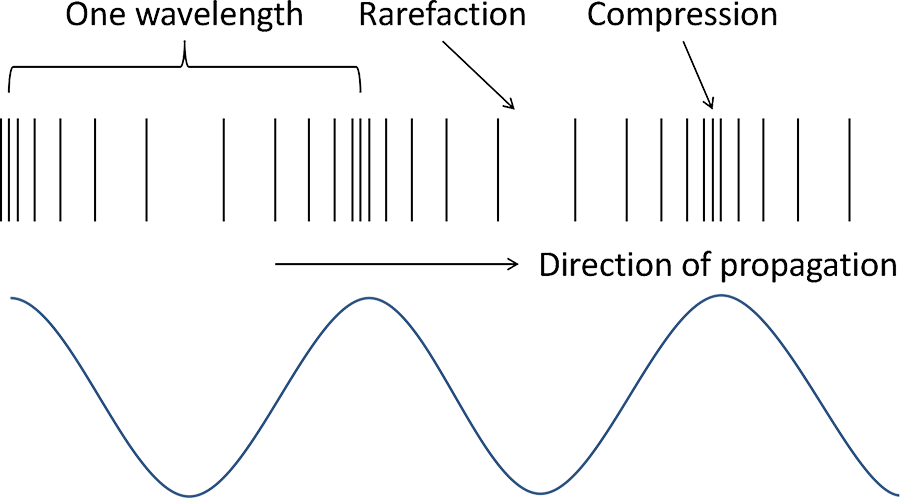
\includegraphics[width=8cm]{sound}
  \caption{Mechanical movement of the particles with the sound
    \cite{abdulla2025properties_sound}.\label{fig:sound}}
\end{figure}

\section{Echoes}
\begin{itemize}
\item (Ultra)Sound waves pass through tissues, get reflected, and the
  returning wave (echo) is detected and forms the image. In
  \popup{B-mode}{B for Brightness (the most common ultrasound imaging
    used in medicine). There is A-Mode (A for Amplitude) that is
    mainly used in ophthalmology to investigate retinal detachment.}
  imaging, the intensity of the returning wave (echo) is represented
  as a level of brightness on the monitor to give a 2D cross-sectional
  image on the monitor \cite{abdulla2025ultrasound} (see Figure
  \ref{fig:interactions}).
\end{itemize}
\vspace{-3ex}
\begin{figure}[!h]
  \centering
  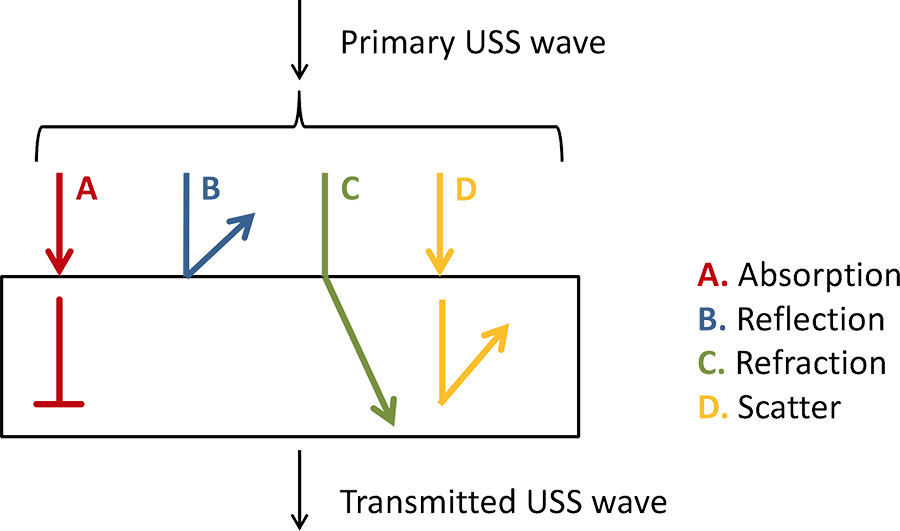
\includegraphics[width=6cm]{sound_interactions}
  \caption{Interactions of the ultrasound scan (USS) with tissue
    \cite{abdulla2025properties_sound}.\label{fig:interactions}}
\end{figure}

\section{Ultrasound imaging with flow detection}

\begin{itemize}
\item The speed of the sound signal in the tissues are low enough to
  use the Doppler effect to detect their motion
  \cite{bushberg2011essential,abdulla2025ultrasound_machine}. Thus,
  for example, using the M-Mode (M for Motion) we can measure the
  blood flow displayed as color channels (see Figure~\ref{fig:doppler}
  ).\footnote{Both the speed and direction of blood flow can be
    measured, and within a subarea of the grayscale image, a color
    flow display typically shows blood flow in one direction as red,
    and in the other direction as blue \cite{bushberg2011essential}.}
\end{itemize}
\vspace{-3ex}
\begin{figure}[!h]
  \centering
  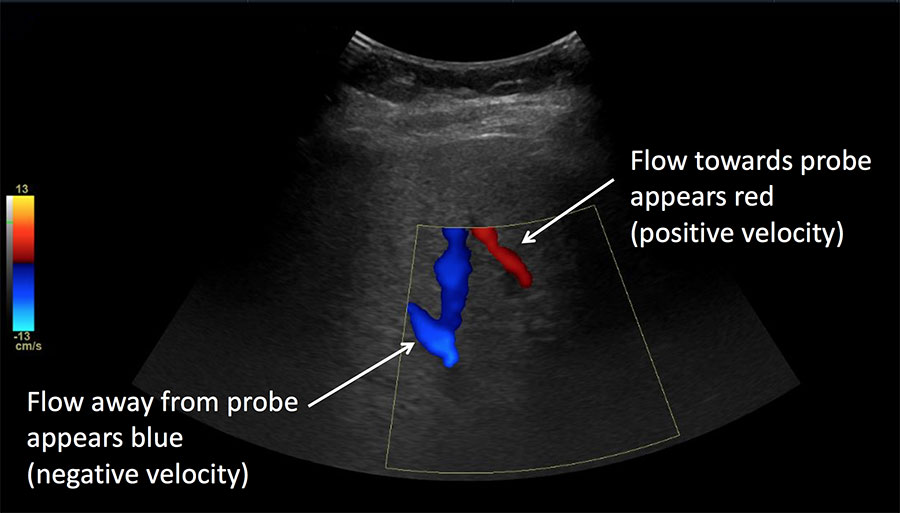
\includegraphics[width=8cm]{doppler}
  \caption{An ultrasound image that shows the Doppler effect
    \cite{abdulla2025ultrasound_imaging_doppler}.\label{fig:doppler}}
\end{figure}

\section{Acquisition details}
The echoes returned are shown on screen in a grey-scale corresponding
to their intensity. The structures are shown as a 2D image on
screen. A short-duration pulse of sound is generated by an ultrasound
transducer that is in direct physical contact with the tissues being
imaged. The sound waves travel into the tissue, and are reflected by
internal structures in the body, creating echoes. The reflected sound
waves then reach the transducer, which records the returning sound
\cite{bushberg2011essential,abdulla2025ultrasound_machine}.



\section{Image content}
Ultrasound imaging is basically a 2D technique (slices). However, 3D
images (volumes) can be generated by placing the known voxels in a 3D
structure and interpolating the unknown voxels. Then, using
segmentation it is possible to display surfaces to see, for example,
the face of a fetus.

\section{Speckle noise}
Ultrasound images are noisy and the predominant type of noise is
speckle noise.

Speckle is usually modeled as multiplicative noise. Amplitude
(magnitude) follows a Rayleigh distribution. Phase is uniformly
distributed. Intensity (amplitude squared) follows an exponential
distribution.

If multiple images are taken (changing the angle and orientation) and
averaged, then intensity in the resulting \emph{spatial compounding}
\cite{bushberg2011essential} follows a Gamma distribution.
